\documentclass[a4paper,11pt, final]{scrartcl}

\usepackage[utf8]{inputenc}
\usepackage[T1]{fontenc}

\usepackage{color}
\usepackage{enumerate}
\usepackage{amsmath}
\usepackage{graphics}
\usepackage{graphicx}
\usepackage{amssymb}
\usepackage{tikz}
\usepackage{marvosym}

\usetikzlibrary{positioning}
\usetikzlibrary{arrows}

\usepackage{fancyhdr}
\pagestyle{fancy}
\fancyhf{}
\markright{headline}

% Hack for the equivalence symbol
\newcommand{\vDashv}{\ensuremath{\vDash \hspace{-0.3cm} \Dashv}}
\newcommand{\todo}[1]{\textcolor{red}{\textbf{TODO }\texttt{#1}}}
\newcommand{\remark}[1]{\textcolor{red}{Remark: \texttt{#1}}}

\begin{document}
\lhead{
    \begin{tabular}{l}
        Probabilistic Graphical Models\\
        WS 2015/16\\
    \end{tabular}
}
\chead{
    Exercise Sheet 5
}
\rhead{
    \begin{tabular}{r}
        Marc Tonsen, 2537359\\
        Franziska Müller, 2542117 
    \end{tabular}
}

\hspace{5cm}

\section*{Exercise 1}

\begin{minipage}{0.5\textwidth}
{
\centering 

\includegraphics[width=0.95\textwidth]{ex2_stripes_ground_truth.png}
\captionof{figure}{Toy stripes}
}  
\end{minipage}
\begin{minipage}{0.5\textwidth}
{
\centering 

\includegraphics[width=0.95\textwidth]{ex2_checker_ground_truth.png}
\captionof{figure}{Toy checkerboard}
}  
\end{minipage}

\section*{Exercise 2}

\begin{minipage}{0.5\textwidth}
{
\centering 

\includegraphics[width=0.95\textwidth]{ex2_stripes_noisy.png}
\captionof{figure}{Noisy toy stripes}
}  
\end{minipage}
\begin{minipage}{0.5\textwidth}
{
\centering 

\includegraphics[width=0.95\textwidth]{ex2_checker_noisy.png}
\captionof{figure}{Noisy toy checkerboard}
}
\end{minipage}

{
\centering 
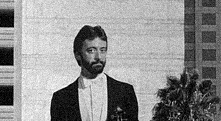
\includegraphics[width=0.32\textwidth]{ex2_image_noisy_less_noise.png}
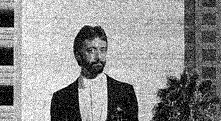
\includegraphics[width=0.32\textwidth]{ex2_image_noisy.png}
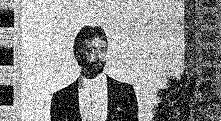
\includegraphics[width=0.32\textwidth]{ex2_image_noisy_more_noise.png}
\captionof{figure}{Image with Gaussian noise and $\sigma = 5$ (left), $\sigma = 25$ (middle) and $\sigma = 50$ (right).}
}

\begin{minipage}{0.5\textwidth}
{
\centering 

\includegraphics[width=0.95\textwidth]{ex2_stripes_median_filter.png}
\captionof{figure}{Noisy toy stripes median filtered.}
}  
\end{minipage}
\begin{minipage}{0.5\textwidth}
{
\centering 

\includegraphics[width=0.95\textwidth]{ex2_checker_median_filter.png}
\captionof{figure}{Noisy toy checkerboard median filtered.}
}  
\end{minipage}

\vspace{1cm}
{
\centering 
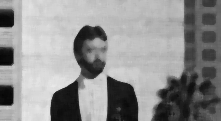
\includegraphics[width=0.32\textwidth]{ex2_image_median_filter_less_noise.png}
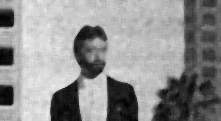
\includegraphics[width=0.32\textwidth]{ex2_image_median_filter.png}
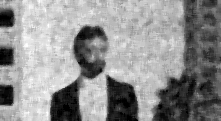
\includegraphics[width=0.32\textwidth]{ex2_image_median_filter_more_noise.png}
\captionof{figure}{Image with Gaussian noise and $\sigma = 5$ (left), $\sigma = 25$ (middle) and $\sigma = 50$ (right) median filtered.}
}

\subsection*{Varying noise for median filter}
We have included noisy images and the corresponding filter results for sigma values 5 and 50. The smaller sigma, the smoother the filtered image becomes. Natural images usually contain smooth areas in which the median filters deletes any high frequencies. If there is a lot of noise in an image the result looks less smooth and more like there is still noise left, which makes sense since also the median in each window can shift significantly if the noise is strong, so there is often a big difference for pixels even with overlapping windows.

\vspace{1cm}
{
\centering 
\begin{tabular}{|c|c|c|c|c|c|} \hline
  & Noisy Original & Median & Gauss MRF & Median + Gauss MRF & Student MRF \\ \hline
 Stripes & 13.3348 & 29.7881 & 18.9248 & 22.5530 & 13.4212 \\ \hline
 Checker & 13.4040 & 26.6421 & 17.9571 & 20.5386 & 13.4872 \\ \hline
 Image & 20.4622 & 24.1984 & 25.0029 & 23.2165 & 23.5804 \\ \hline
\end{tabular}
\captionof{table}{PSNR Ex 2 and Ex 3}
}  

\section*{Exercise 3}

\subsection*{Parameter Tuning}
We picked $\sigma$ as 10 and $\eta$ as 0.1. For bigger sigma the images tend to not get denoised at all. For smaller sigma the computed result is very far off from the ground truth image. For smaller values of eta the gradient ascent did not always converge. For bigger values of eta the gradient ascent converged quicker, but the achieved PSNR value of the result was lower.

\subsection*{Median filter vs Gauss MRF}
For the salt and pepper noise the median filter works a lot better, which makes sense since this kind of noise only affects a few single pixes, which leaves the median in the filtering window mostly intact. The Gauss MRF only adds blur to the images resulting in no great effect. On the natural image the median filter adds a lot of blur, deleting all the noise but also many image features. The Gauss MRF works better on natural images, leaving more image features intact. These observations are verified if one consideres the PSNR values, which also indicate that for the salt and pepper noise the Median filter is better and for the gaussian noise the Gauss MRF is better.

\subsection*{Initializing gradient ascent with the result of the median filter}
According to the PSNR values this approach works better for the artificial videos and worse for the real image. The visual impression for us was mostly an additional slight blur in all cases. In terms of performance the gradient ascent converged slower if we initialized it with the result of the median filter in all cases.

\vspace{1cm}
{
\centering 
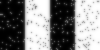
\includegraphics[width=0.48\textwidth]{ex3_stripes_mrf_gaussian_filter.png}
\hfill
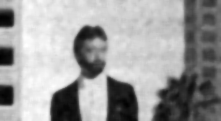
\includegraphics[width=0.48\textwidth]{ex3_stripes_median_into_mrf_gaussian_filter.png}
\captionof{figure}{Noisy stripes filtered with MRF Gaussian (left) and filtered with MRF Gaussian initialized with Median Filter result.}
}

{
\centering 
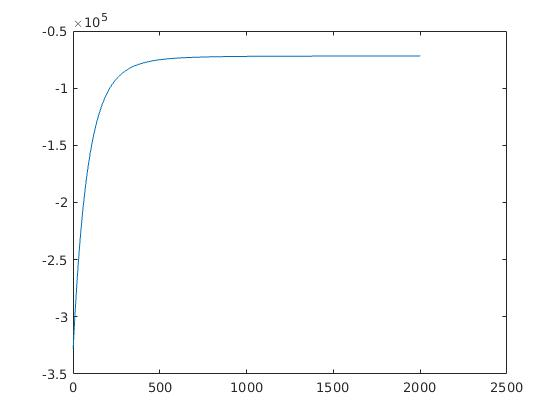
\includegraphics[width=0.48\textwidth]{ex3_stripes_gauss_mrf_posterior.jpg}
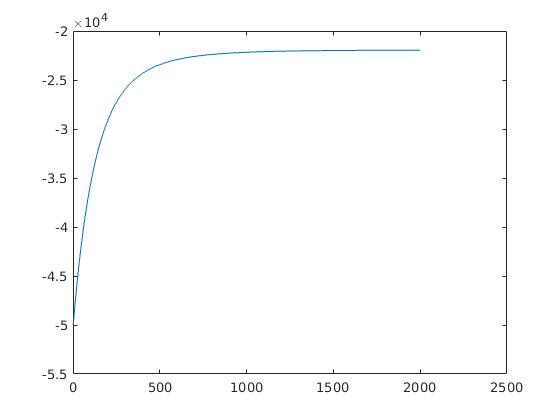
\includegraphics[width=0.48\textwidth]{ex3_stripes_median_into_gauss_mrf_posterior.jpg}
\captionof{figure}{Posterior curve for noisy stripes filtered with MRF Gaussian (left) and filtered with MRF Gaussian initialized with Median Filter result.}
}

{
\centering 
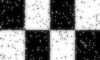
\includegraphics[width=0.48\textwidth]{ex3_checker_mrf_gaussian_filter.png}

\includegraphics[width=0.48\textwidth]{ex3_checker_median_into_mrf_gaussian_filter.png}
\captionof{figure}{Noisy checkerboard filtered with MRF Gaussian (left) and filtered with MRF Gaussian initialized with Median Filter result.}
}

{
\centering 
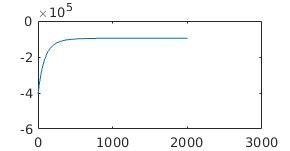
\includegraphics[width=0.48\textwidth]{ex3_checker_gauss_mrf_posterior.jpg}
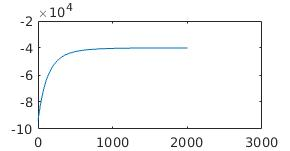
\includegraphics[width=0.48\textwidth]{ex3_checker_median_into_gauss_mrf_posterior.jpg}
\captionof{figure}{Posterior curve for noisy checkerboard filtered with MRF Gaussian (left) and filtered with MRF Gaussian initialized with Median Filter result.}
}

{
\centering 
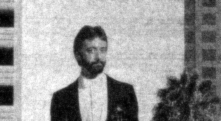
\includegraphics[width=0.48\textwidth]{ex3_image_mrf_gaussian_filter.png}
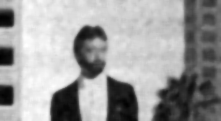
\includegraphics[width=0.48\textwidth]{ex3_image_median_into_mrf_gaussian_filter.png}
\captionof{figure}{Noisy image filtered with MRF Gaussian (left) and filtered with MRF Gaussian initialized with Median Filter result.}
}

{
\centering 
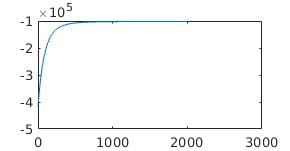
\includegraphics[width=0.48\textwidth]{ex3_image_gauss_mrf_posterior.jpg}
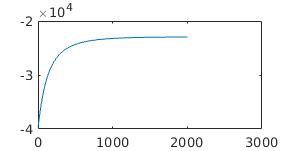
\includegraphics[width=0.48\textwidth]{ex3_image_median_into_gauss_mrf_posterior.jpg}
\captionof{figure}{Posterior Curve for noisy image filtered with MRF Gaussian (left) and filtered with MRF Gaussian initialized with Median Filter result.}
}

\section*{Exercise 4}
\subsection*{Convergence}
The overall convergence is slower than when using the Gaussian prior in exercise 3. It takes the full 2000 iterations to approximately converge. 

{
\centering 
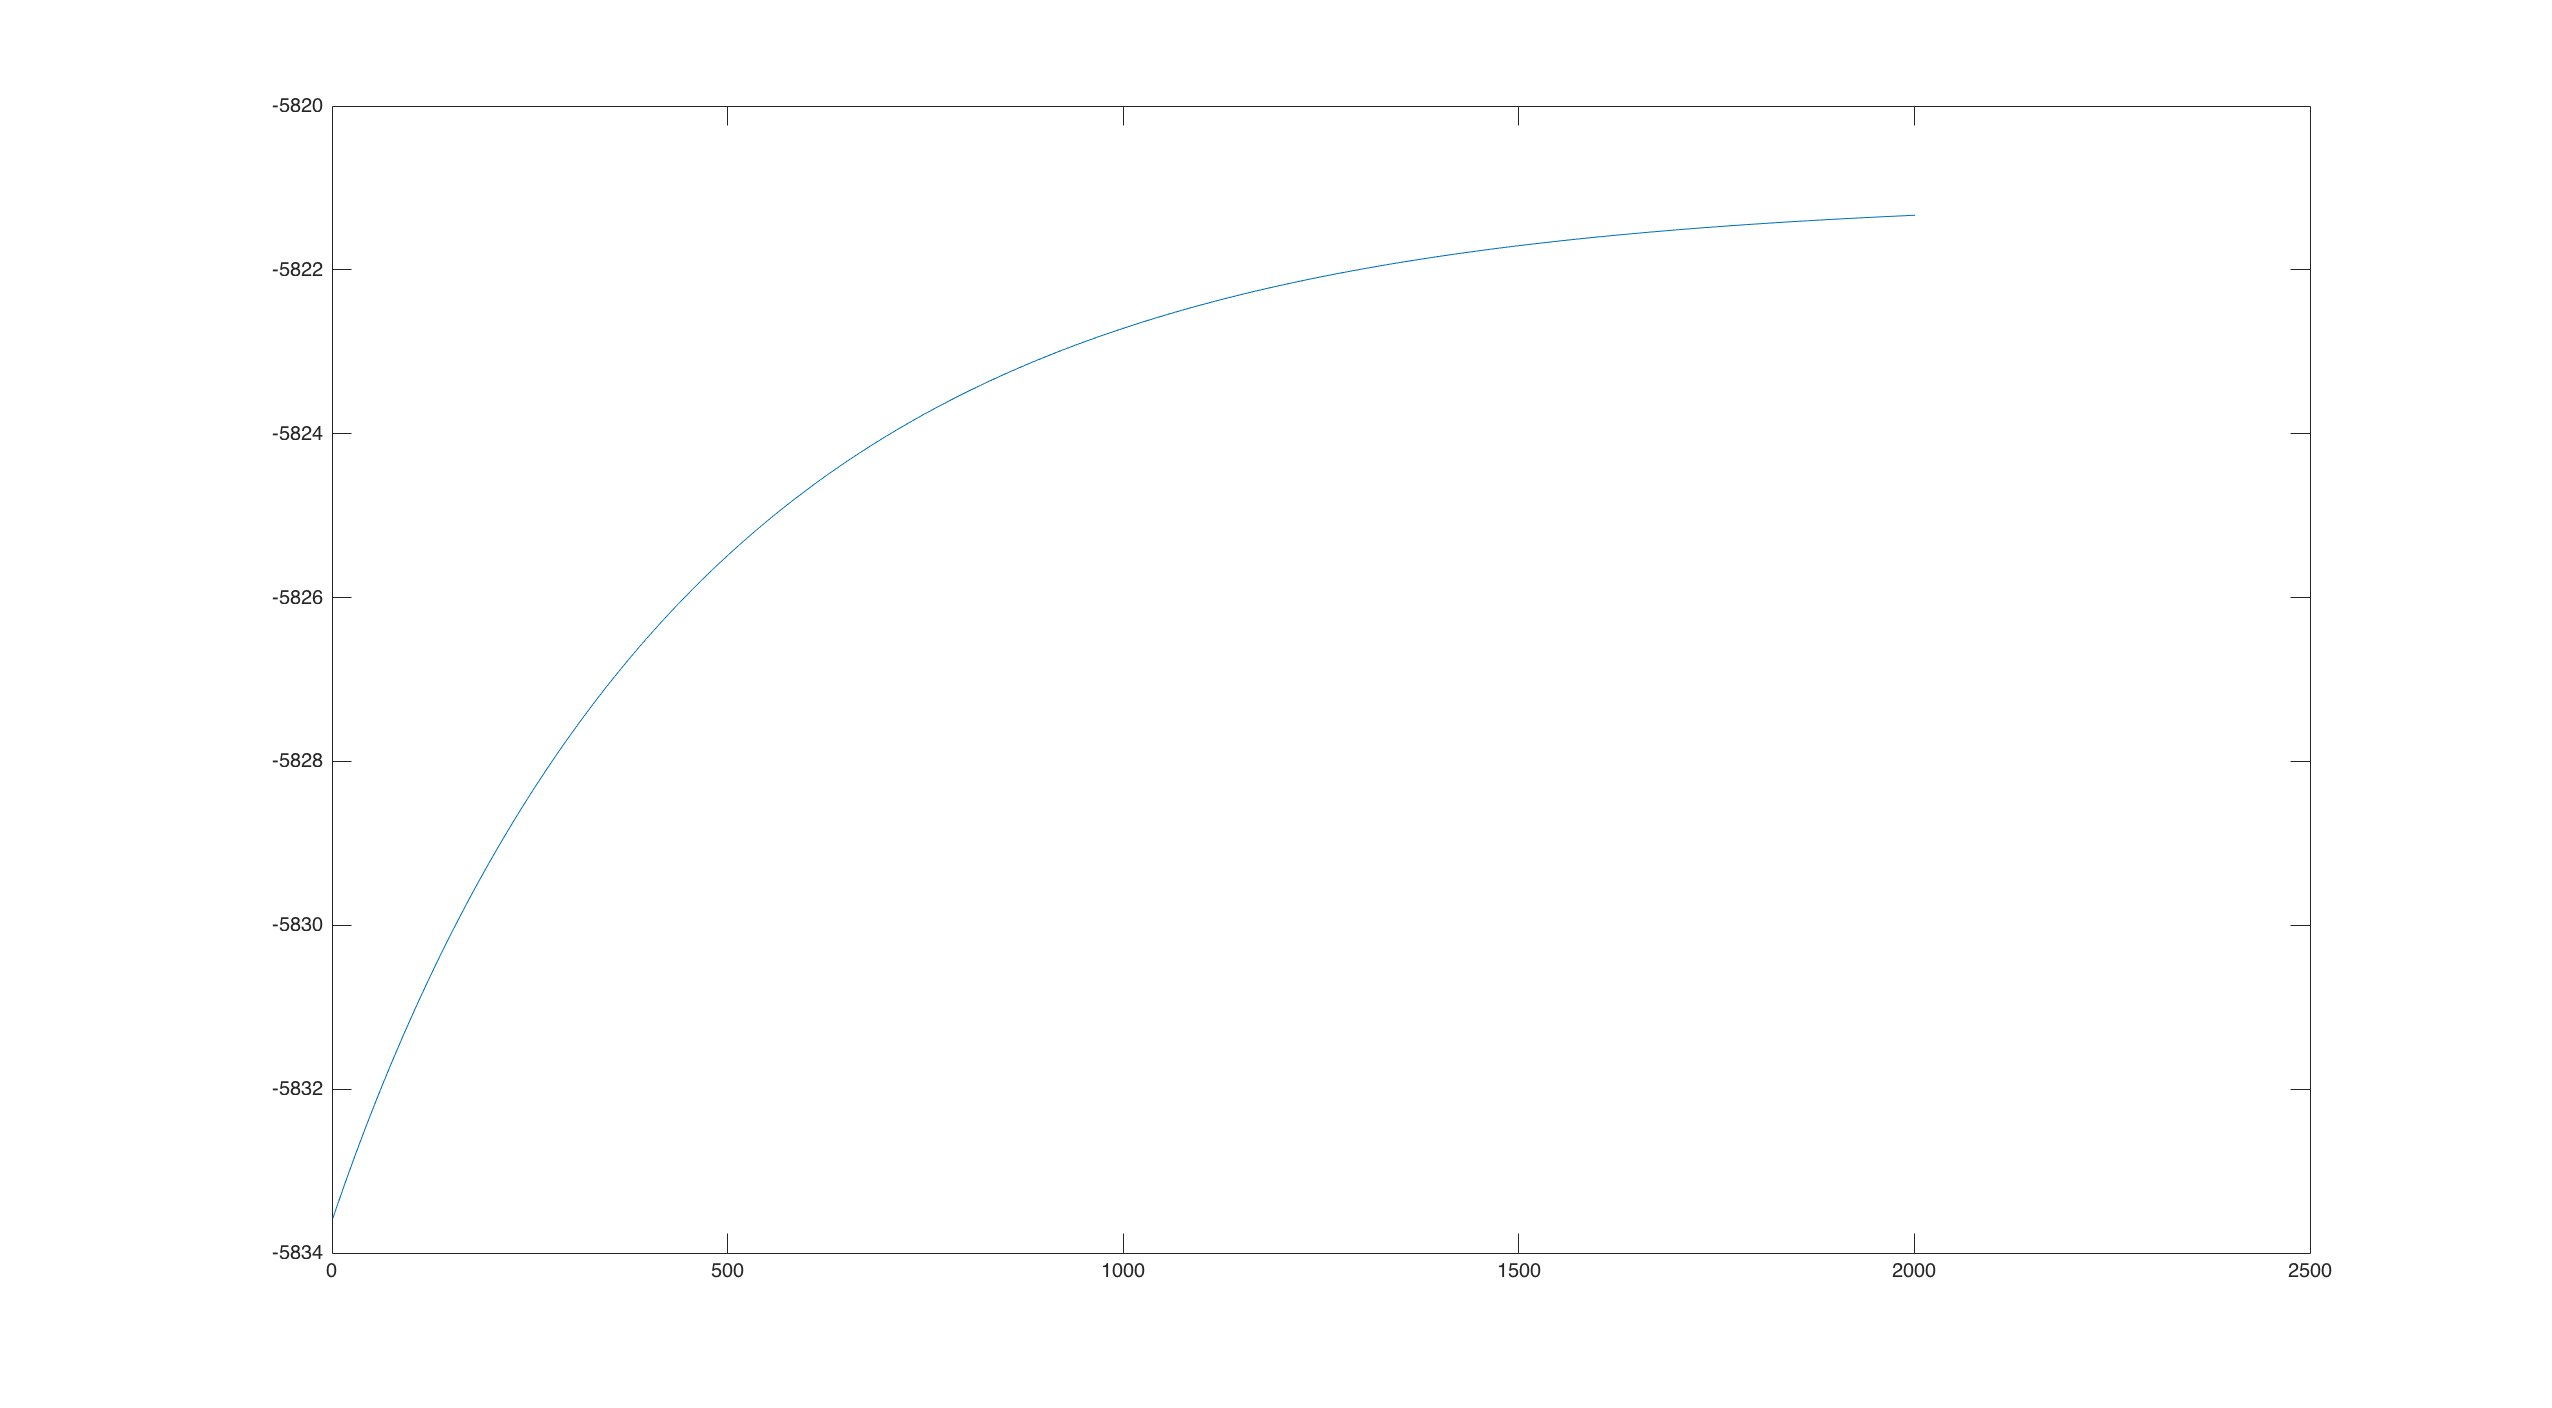
\includegraphics[width=0.32\textwidth]{ex4_stripes_mrf_student_posterior.png}
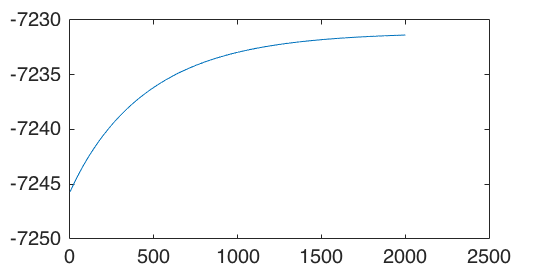
\includegraphics[width=0.32\textwidth]{ex4_checker_mrf_student_posterior.png}
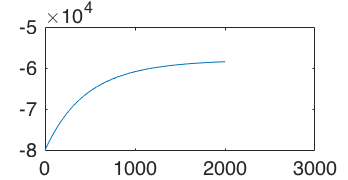
\includegraphics[width=0.32\textwidth]{ex4_image_mrf_student_posterior.png}
\captionof{figure}{Increasing log-posterior curve for stripes (left), checkerboard (middle) and image (right) using MRF Student Filter.}
}

\vspace{1cm}

{
\centering 

\includegraphics[width=0.32\textwidth]{ex4_stripes_mrf_student_filtered.png}

\includegraphics[width=0.32\textwidth]{ex4_checker_mrf_student_filtered.png}
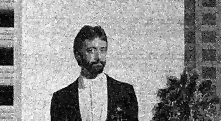
\includegraphics[width=0.32\textwidth]{ex4_image_mrf_student_filtered.png}
\captionof{figure}{Denoising results for stripes (left), checkerboard (middle) and image (right) using MRF Student Filter.}
}

\subsection*{Performance}
Although there is a slight improvement in PSNR when denoising the artifical images, this difference is not visible when looking at the images. This can be explained by the fact that the Student-t prior is suited for natural images but not for artificial ones.
For the real image, the PSNR improves significantly. The difference is also visible when comparing the images. Overall, the result is less noisy and especially not as blurry as the result when using the Gaussian prior. Edges and also face features are maintained better.

{
\centering 
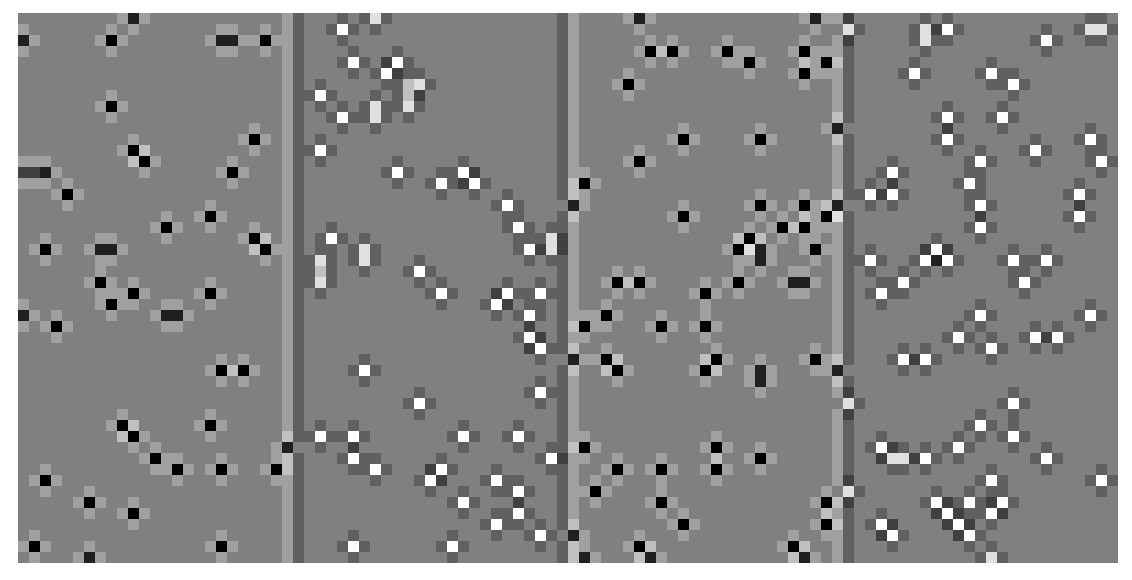
\includegraphics[width=0.32\textwidth]{ex4_stripes_grad.png}
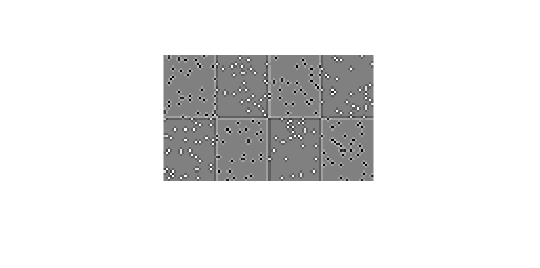
\includegraphics[width=0.32\textwidth]{ex4_checker_grad.png}
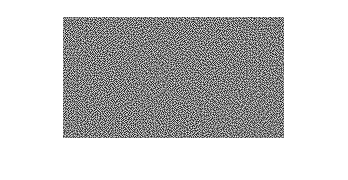
\includegraphics[width=0.32\textwidth]{ex4_image_grad.png}
\captionof{figure}{Gradients of the log-prior for stripes (left), checkerboard (middle) and image (right) using MRF Student Filter.}
}

\vspace{1cm}

\subsection*{Gradients of the student prior}
\begin{itemize}
\item artificial images: The gradient of the student prior has a high absolute value in the noisy pixels. The direction of the gradient is opposite for noisy salt-pixels in a black area and noisy pepper-pixels in a white area of the image. That is because the pixel values have to change in opposite directions (increase, decrease) to achieve a better value in the student prior that wants to make pixels similar to their neighbors. Therefore, also the gradient at the edges of the stripes or the checkerboard is stronger but not as strong as in the noisy pixels since roughly half of the neighbors have the same color.
\item real image: The gradient in the real image looks in most regions more or less random what also makes sense because the Gaussian noise was random. Only in edge regions, the gradient is significantly less strong. That matches the result that the edges are less blurry when using this filtering technique.  
\end{itemize}

\section*{Exercise 5}
\subsection*{Reasonable assumption?}
This depends on the noise type that is present in the image. Noise can be added for example as salt-and-pepper noise caused by transmission errors or defects in the camera sensor. In this case, only some pixels are affected randomly and therefore the noise is independent.
In the digitization of old movies, film grain noise occurs in lines, so the noise is not independent.
Overall, in many applications the assumption is reasonable.

\subsection*{What happens?}
\begin{itemize}
\item Gaussian prior: When using the Gaussian prior, the whole image is blurred. This reduces the noise in the area of the stripe but blurrs also all edges in the remaining image.
\item Student prior: Noisy pixels whose values do not differ so much from the true value are denoised properly. More intense noise remains. But other regions of the images (not affected by the noisy stripe) are barely changed.  
\end{itemize}

{
\centering 

\includegraphics[width=0.32\textwidth]{ex5_stripes_noise.png}
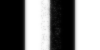
\includegraphics[width=0.32\textwidth]{ex5_stripes_mrf_gaussian_filtered.png}
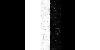
\includegraphics[width=0.32\textwidth]{ex5_stripes_mrf_student_filtered.png}
\captionof{figure}{Gradients of the log-prior for stripes (left), checkerboard (middle) and image (right) using MRF Student Filter.}
}

{
\centering 
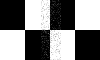
\includegraphics[width=0.32\textwidth]{ex5_checker_noise.png}
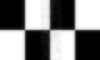
\includegraphics[width=0.32\textwidth]{ex5_checker_mrf_gaussian_filtered.png}
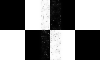
\includegraphics[width=0.32\textwidth]{ex5_checker_mrf_student_filtered.png}
\captionof{figure}{Gradients of the log-prior for stripes (left), checkerboard (middle) and image (right) using MRF Student Filter.}
}

{
\centering 
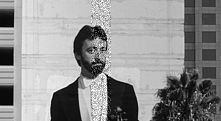
\includegraphics[width=0.32\textwidth]{ex5_image_noise.png}
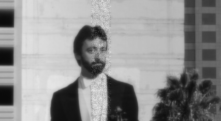
\includegraphics[width=0.32\textwidth]{ex5_image_mrf_gaussian_filtered.png}
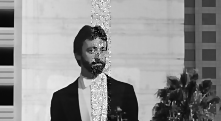
\includegraphics[width=0.32\textwidth]{ex5_image_mrf_student_filtered.png}
\captionof{figure}{Gradients of the log-prior for stripes (left), checkerboard (middle) and image (right) using MRF Student Filter.}
}

\section*{Exercise 6}
There are several ways to denoise a color image.
One idea is to denoise the different channels of the image separately using the same techniques that we used for grey value images.
One could also use another color space, like HSV, where the color can be more easily split into color and brightness information (color noise is more disturbing than brightness noise for the human). 

\end{document}
